\begin{center}
    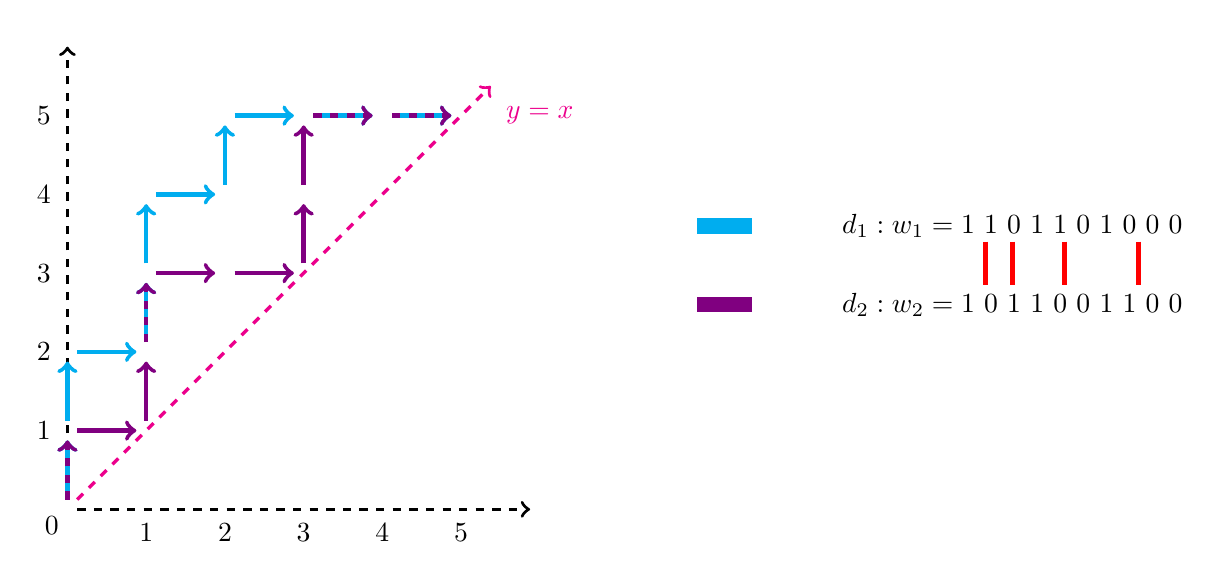
\begin{tikzpicture}[scale=1]
        \node (a) at (0, 0) {};
        \node (b) at (0, 6) {};
        \node (c) at (6, 0) {};
        \node (d) at (5.5, 5.5) {};
        \node (e) at (6, 5) [color = magenta] {$y = x$}; 
        \draw [dashed, very thick, ->] (a) to (b);
        \draw [dashed, very thick, ->] (a) to (c);
        \draw [dashed, very thick, ->]
            [color = magenta] (a) to (d);

        \node (1)  at (0,0)   {};
        \node (2)  at (0,1)   {};
        \node (3)  at (0,2)   {};
        \node (3b) at (1, 1)  {};
        \node (4)  at (1,2)   {};
        \node (5)  at (1,3)   {};
        \node (6)  at (1,4)   {};
        \node (6b) at (2,3)   {};
        \node (7)  at (2,4)   {};
        \node (7b) at (3,3)   {};
        \node (8)  at (2,5)   {};
        \node (8b) at (3, 4)  {};
        \node (9)  at (3,5)   {};
        \node (10) at (4,5)   {};
        \node (11) at (5,5)   {};

        \draw [->, ultra thick, color = cyan]
            (1)  to (2);
        \draw [->, ultra thick, color = cyan] 
            (2)  to (3);
        \draw [->, ultra thick, color = cyan]
            (3)  to (4);
        \draw [->, ultra thick, color = cyan]
            (4)  to (5);
        \draw [->, ultra thick, color = cyan]
            (5)  to (6);
        \draw [->, ultra thick, color = cyan]
            (6)  to (7);
        \draw [->, ultra thick, color = cyan]
            (7)  to (8);
        \draw [->, ultra thick, color = cyan]
            (8)  to (9);
        \draw [->, ultra thick, color = cyan]
            (9)  to (10);
        \draw [->, ultra thick, color = cyan]
            (10) to (11);

        \draw [->, dashed, ultra thick, color = violet]
            (1)  to (2);
        \draw [->, ultra thick, color = violet] 
            (2)  to (3b);
        \draw [->, ultra thick, color = violet]
            (3b)  to (4);
        \draw [->, dashed, ultra thick, color = violet]
            (4)  to (5);
        \draw [->, ultra thick, color = violet]
            (5)  to (6b);
        \draw [->, ultra thick, color = violet]
            (6b)  to (7b);
        \draw [->, ultra thick, color = violet]
            (7b)  to (8b);
        \draw [->, ultra thick, color = violet]
            (8b)  to (9);
        \draw [->, dashed, ultra thick, color = violet]
            (9)  to (10);
        \draw [->, dashed, ultra thick, color = violet]
            (10) to (11);

        \node at (-0.2, -0.2) {$0$};
        \node at (-0.3, 1)    {$1$};
        \node at (1, -0.3)    {$1$};
        \node at (-0.3, 2)    {$2$};
        \node at (2, -0.3)    {$2$};
        \node at (-0.3, 3)    {$3$};
        \node at (3, -0.3)    {$3$};
        \node at (-0.3, 4)    {$4$};
        \node at (4, -0.3)    {$4$};
        \node at (-0.3, 5)    {$5$};
        \node at (5, -0.3)    {$5$};

    \fill[color = cyan] (8,3.5) rectangle (8.7,3.7);
    \node at (12,3.6) {$d_1 : w_1 = 1\ 1\ 0\ 1\ 1\ 0\ 1\ 0\ 0\ 0$};
    \fill[color = violet] (8,2.5) rectangle (8.7,2.7);
    \node at (12,2.6) {$d_2 : w_2 = 1\ 0\ 1\ 1\ 0\ 0\ 1\ 1\ 0\ 0$};

    \draw [-, ultra thick, color = red] (11.66,3.4) to (11.66,2.85);
    \draw [-, ultra thick, color = red] (12,3.4) to (12,2.85);
    \draw [-, ultra thick, color = red] (12.66,3.4) to (12.66,2.85);
    \draw [-, ultra thick, color = red] (13.6,3.4) to (13.6,2.85);

    \end{tikzpicture}
\end{center}